\documentclass[11pt,a4paper]{article}
\usepackage[margin=25mm]{geometry}
\usepackage[T1]{fontenc}
\usepackage{lmodern,microtype}
\usepackage{amsmath,amssymb,amsthm,mathtools}
\usepackage{booktabs,array,graphicx,xcolor}
\usepackage{enumitem}
\usepackage[colorlinks=true,linkcolor=violet!65!black,citecolor=violet!65!black,urlcolor=violet!65!black]{hyperref}
\newtheorem{theorem}{Theorem}[section]
\newtheorem{lemma}[theorem]{Lemma}
\newtheorem{proposition}[theorem]{Proposition}
\newtheorem{corollary}[theorem]{Corollary}
\theoremstyle{definition}
\newtheorem{definition}[theorem]{Definition}
\theoremstyle{remark}
\newtheorem{remark}[theorem]{Remark}
\newcommand{\Prb}{\mathbb P}
\newcommand{\E}{\mathbb E}
\newcommand{\Bin}{\operatorname{Bin}}
\newcommand{\tr}{\operatorname{tr}}
\newcommand{\avd}{\operatorname{avd}}
\newcommand{\Ent}{\operatorname{Ent}}
\newcommand{\cA}{\mathcal A}
\newcommand{\cC}{\mathcal C}
\hypersetup{pdftitle={Domination polynomials with many peaks},pdfauthor={Anonymous}}
\title{Domination polynomials with many peaks\\[5pt]
\large Counterexamples to the Alikhani--Peng conjecture\\
and the minimum-degree scale for a central mode}
\author{Anonymous}
\date{November 2026\\[2pt]\small DOI \href{https://doi.org/10.5281/zenodo.24511988}{10.5281/zenodo.24511988}}
\begin{document}
\maketitle

\begin{abstract}
A set of vertices of a graph dominates it when every vertex is in the set or next to it. Counting dominating sets by size gives a sequence $d_0,d_1,\dots,d_n$, the coefficients of the domination polynomial. In 2009 Alikhani and Peng conjectured that this sequence is always unimodal: it rises to a maximum and then falls. The conjecture has been proved for many graph classes and for graphs of minimum degree at least $2\log_2 n$, and it was still listed as open in 2026. We show that it is false. Two explicit graphs on $317\,440$ vertices, one split and one bipartite, satisfy $d_{160080}>d_{160320}<d_{160560}$; an integer-arithmetic certificate proves the three inequalities. The mechanism is phase coexistence: two large families of dominating sets have exactly the same number of members but different typical sizes. The same idea gives connected graphs with order $\sqrt n/\log n$ separated peaks, and graphs in which every most frequent size is at distance of order $n$ from the average size, which answers a question of Beaton and Brown; for the explicit $317\,440$-vertex split graph no index within distance $88$ of the average size is a most frequent size. Counterexamples persist at minimum degree $(\tfrac12+o(1))\log_2 n$. In the positive direction, a double count of one-vertex additions shows that $\sum_v(\deg v+2)2^{-\deg v-1}\le1$ forces unimodality with the maximum at $\lceil n/2\rceil$. Hence minimum degree $\log_2n+\log_2\log_2n+1$ suffices for this conclusion, and for every large $n$ this is best possible up to an additive constant. Whether minimum degree $(1-\varepsilon)\log_2 n$ already forces unimodality remains open.
\end{abstract}

\section{Introduction}\label{sec:intro}
This section explains the problem, what was known, what is new and how the paper is organised.

\subsection{The problem}
All graphs are finite, simple and undirected; $n$ denotes the number of vertices. A set $S\subseteq V(G)$ \emph{dominates} $G$ when every vertex lies in $S$ or has a neighbour in $S$. Equivalently, $S$ meets every closed neighbourhood $N[v]=\{v\}\cup N(v)$. Write
\[
d_k(G)=\#\{S\subseteq V(G):S\text{ dominates }G,\ |S|=k\},
\qquad D_G(z)=\sum_{k=0}^{n}d_k(G)z^k .
\]
The polynomial $D_G$ is the \emph{domination polynomial}. A sequence is \emph{unimodal} when it weakly increases up to some index and weakly decreases thereafter. Unimodality and the stronger log-concavity are basic shape questions for graph polynomials, and for several of them, including this one, they remain largely open.

Alikhani and Peng introduced the domination polynomial and stated the conjecture that \emph{the domination polynomial of any graph is unimodal} \cite[p.~7]{AP}. The question has a probabilistic reading that we use throughout: if a dominating set is chosen uniformly at random, $d_k(G)/D_G(1)$ is the probability that it has size $k$, so the conjecture says the size distribution of a uniform dominating set never has two separated humps.

\subsection{What was known}
Adding a vertex to a dominating set keeps it dominating, and a simple injection shows $d_k\le d_{k+1}$ for every $k<n/2$ \cite[Proposition~2.4]{BB}. Any failure of unimodality must therefore occur in the upper half of the sequence. Beaton and Brown also remark that for graphs without isolated vertices the coefficients do not increase from $\lfloor3n/4\rfloor$ onwards \cite[Section~4]{BB}. Burcroff and O'Brien prove that a portion of every such sequence is nonincreasing, of a length that depends on the upper domination number, and prove unimodality for several families, including spiders with at most $400$ legs \cite{BO}.

The conjecture is known for paths, cycles and complete multipartite graphs \cite{BB}, for the families just mentioned \cite{BO}, for powers of paths and cycles \cite{GZ}, for threshold graphs (with log-concavity) \cite{Omar}, and for large graphs with a universal vertex \cite{Zhang}. Beaton and Brown proved it for all graphs of minimum degree $\delta\ge2\log_2 n$, with the maximum at $\lceil n/2\rceil$ \cite[Theorem~3.2]{BB}; Omar gave the variant $\delta\ge\log_2(n(n+2))-2$ \cite[Proposition~13]{Omar}. On the negative side, log-concavity can fail: Beaton and Schoonhoven found trees with non-log-concave domination polynomials \cite{BS}, and Du, Heilman and Panova found trees with arbitrarily many failures of log-concavity \cite{DHP}. Both papers, and Omar's, describe unimodality itself as open, even for trees. Omar also asks whether total positivity can prove unimodality for split graphs \cite[Section~6, question~(3)]{Omar}. Finally, Beaton and Brown ask whether the maximum is always at one of the two integers next to the average size $\avd(G)=D_G'(1)/D_G(1)$ of a dominating set, and if not, how far apart the two can be \cite[Section~4]{BB}.

For independent sets the analogous story is older. Bhattacharyya and Kahn disproved the Levit--Mandrescu conjecture that bipartite graphs have unimodal independent-set sequences \cite{BK}. Their graph has two families of independent sets of comparable total size whose sizes concentrate at different values, and the sequence dips between the two. Our construction follows the same principle. The new difficulty is that domination is a covering condition rather than a packing condition: every vertex must be covered, so two families cannot simply be placed side by side. The gadget below arranges the covering constraints so that the two families have \emph{exactly} equal size while everything else is negligible.

\subsection{Results}
We use \emph{global mode} for an index $k$ at which $d_k$ is largest, and \emph{peak region} for a maximal run of indices forming a local maximum (a plateau is allowed) that is separated from the next such run by a strictly lower coefficient.

\begin{theorem}[An explicit counterexample]\label{thm:finite}
There is a connected split graph $G$ and a connected bipartite graph $B$, each on $317\,440$ vertices, for which
\[
d_{160080}>d_{160320}<d_{160560}.
\]
Every vertex in one independent part of each graph has degree three. The bipartite graph has maximum degree $120$.
\end{theorem}

\begin{theorem}[Many peaks]\label{thm:many-summary}
Along infinite sequences of orders $n$, connected split graphs and connected bipartite graphs have at least $c\sqrt n/\log n$ peak regions, for an absolute constant $c>0$. The bipartite examples have maximum degree $O(\log n)$. Explicitly, there are such graphs with four peak regions on $4\,857\,004\,032$ vertices.
\end{theorem}
Bhattacharyya and Kahn remark that their construction extends to give independent-set sequences of bipartite graphs with arbitrarily many local maxima \cite[Section~3]{BK}; Theorem~\ref{thm:many-summary} is the analogue for dominating sets, with a quantitative count.

\begin{theorem}[Modes far from the average]\label{thm:mean-summary}
\begin{enumerate}[label=(\alph*)]
\item There is an absolute constant $c>0$ such that, for connected split graphs and for connected bipartite graphs of infinitely many orders $n$, every global mode $j$ satisfies $|j-\avd(G)|\ge cn$.
\item For the split graph $G$ of Theorem~\ref{thm:finite}, $160323.034984\le\avd(G)\le 160323.034985$, and $d_k(G)$ is not the largest coefficient for any $k$ with $160217\le k\le 160412$. Thus every global mode of $G$ differs from $\avd(G)$ by more than $88$.
\end{enumerate}
\end{theorem}
Part (b) answers the first half of the Beaton--Brown question with an explicit graph. Part (a) answers the second half: the distance can be linear in $n$, which is the largest possible order. The constant in (a) is tiny (Remark~\ref{rem:constants}).

\begin{theorem}[Minimum degree]\label{thm:degree-summary}
The following assertions hold.
\begin{enumerate}[label=(\roman*)]
\item There are connected split graphs and connected bipartite graphs with nonunimodal domination sequences and $\delta(G)/\log_2|V(G)|\to\tfrac12$.
\item Every $n$-vertex graph satisfying
\[
\sum_{v\in V(G)}(\deg(v)+2)2^{-\deg(v)-1}\le1
\]
has a unimodal domination sequence with a global mode at $\lceil n/2\rceil$. In particular this holds whenever $n\ge4$ and $\delta(G)\ge\log_2n+\log_2\log_2n+1$.
\item Let $c(n)$ be the least integer $d$ such that every $n$-vertex graph of minimum degree at least $d$ has a unimodal domination sequence with a global mode at $\lceil n/2\rceil$. Writing $L=\log_2 n$,
\begin{align*}
L+\log_2L-3\le c(n)&\le L+\log_2 L+2&&\text{for even }n\ge2^{20},\\
L+\log_2L-4\le c(n)&\le L+\log_2 L+2&&\text{for odd }n\ge2^{40}.
\end{align*}
\end{enumerate}
\end{theorem}
Part (iii) concerns the \emph{central} mode only. The graphs giving its lower bound have $d_{\lceil n/2\rceil}<d_{\lceil n/2\rceil+1}$, so their largest coefficient is not at $\lceil n/2\rceil$, but they may well be unimodal. For unimodality itself, parts (i) and (ii) place the least sufficient minimum degree between $(\tfrac12+o(1))\log_2n$ and $\log_2 n+\log_2\log_2 n+1$; closing this gap is the main open problem left here.

\subsection{The idea}
Each construction contains two large families of dominating sets with three properties. The two families have exactly the same number of members. Within each family the size of a uniform member is a sum of many independent pieces, so it concentrates around a mean, and the two means differ by much more than the standard deviations. Every dominating set outside the two families belongs to a collection that is negligible in total. The size distribution of a uniform dominating set is then close to an equal mixture of two well-separated humps, and the coefficient between the humps is smaller than the coefficients at the humps. The work lies in building graphs where all three properties hold and can be checked exactly.

\subsection{Roadmap}
Section~\ref{sec:construction} builds the basic graphs and their two families. Section~\ref{sec:certificate} proves Theorem~\ref{thm:finite} with an exact certificate and proves part (b) of Theorem~\ref{thm:mean-summary}. Section~\ref{sec:elementary} gives a computer-free proof of nonunimodality for a larger graph. Section~\ref{sec:many} proves Theorem~\ref{thm:many-summary}, Section~\ref{sec:mode} proves part (a) of Theorem~\ref{thm:mean-summary} and deduces slow mixing of a natural sampler, and Section~\ref{sec:highdegree} proves Theorem~\ref{thm:degree-summary}(i). Section~\ref{sec:upper} proves the sufficient criterion (ii), and Section~\ref{sec:central} proves the lower bounds in (iii). Section~\ref{sec:scope} lists open problems and describes the verification.

\paragraph{Notation.} $\Bin(N,p)$ is a binomial random variable; independent summands are written as sums. $\binom{N}{k}=0$ when $k<0$ or $k>N$. Logarithms without base are natural; $\Ent(u)=-u\log u-(1-u)\log(1-u)$ and $\Ent_2(u)=\Ent(u)/\log 2$. Symbols introduced inside one section are local to that section unless stated otherwise.

\section{The basic construction and its two phases}\label{sec:construction}
This section defines the graphs $G_{m,s}$ and $B_{m,s}$, writes their domination polynomials in terms of the selected ``variable'' vertices, and identifies the two families that drive every counterexample.

Fix integers $m\ge2$ and $s\ge1$, and read indices modulo $m$. For each $i$, let $L_i$ consist of $s$ labelled single vertices (\emph{singletons}) and let $R_i$ consist of $s$ disjoint labelled \emph{triples} of vertices. These $4ms$ vertices are the \emph{variable vertices}; write $V_{\rm var}$ for their set. For every triple $Y$ in $R_i$, every singleton $u$ in $L_i\cup L_{i+1}$ and each two-element subset $Q\subset Y$, add a new vertex adjacent precisely to $u$ and the two elements of $Q$. These are the \emph{clause vertices}; distinct triples $(u,Y,Q)$ give distinct clause vertices. Set
\[
h=ms,\qquad P=6ms^2,\qquad N=P+4h,
\]
so there are $P$ clause vertices and $N$ vertices in all.

The bipartite graph $B_{m,s}$ has just these edges. The split graph $G_{m,s}$ additionally has all edges between variable vertices. The bipartite graph is connected because consecutive blocks share singletons and each clause joins its singleton to two vertices of a triple. In $B_{m,s}$ singletons have degree $6s$, triple vertices have degree $4s$, and every clause has degree three.

\paragraph{The domination polynomial of the split graph.}
Fix a set $S$ of selected variable vertices and let $F=F(S)$ count the clauses with no neighbour in $S$. Each of these $F$ clauses must be selected, and the remaining $P-F$ clauses are free. In the split graph these conditions are also sufficient: a nonempty $S$ dominates all variables through the clique, and when $S$ is empty every clause is forced and every variable has a selected clause neighbour. Consequently
\begin{equation}\label{eq:exactpoly}
D_{G_{m,s}}(z)=
\sum_{S\subseteq V_{\rm var}}z^{|S|+F(S)}(1+z)^{P-F(S)} .
\end{equation}

\paragraph{Bad objects and forcing.} Call an omitted singleton \emph{bad}, and call a triple \emph{bad} when at most one of its vertices is selected. Each triple has four good selections (two or three vertices selected) and four bad ones. A bad singleton next to a bad triple forces one clause when the triple has one selected vertex and three clauses when the triple is empty; good triples and selected singletons force nothing.

\paragraph{The two phases.}
Consider the following two families of dominating sets of $G_{m,s}$.
\begin{itemize}
\item $\cA$: every singleton is selected; triple vertices and clauses are arbitrary.
\item $\cC$: every triple has a good selection; singletons and clauses are arbitrary.
\end{itemize}
In both families no clause is forced, so membership depends only on the variable selection and the clauses are free fair bits. The two families have the same size, and their intersection is small:
\[
|\cA|=|\cC|=H:=2^{P+3h},\qquad |\cA\cap\cC|=H2^{-h}.
\]
The size of a uniform member of each family has the respective distribution
\begin{align}
X_{\cA}&=h+\Bin(P+3h,1/2),\label{eq:phaseA}\\
X_{\cC}&=2h+\Bin(P+h,1/2)+\Bin(h,1/4).\label{eq:phaseB}
\end{align}
Their means differ by $\Delta=h/4$:
\begin{equation}\label{eq:means}
\mu_{\cA}=P/2+5h/2,\quad
\mu_{\cC}=P/2+11h/4,\quad
\Delta=\mu_{\cC}-\mu_{\cA}=h/4.
\end{equation}
Both variances are at most
\begin{equation}\label{eq:variance}
V=P/4+h=\tfrac32ms^2+ms.
\end{equation}
The standard deviation is of order $\sqrt m\,s$, while $\Delta$ is of order $ms$; this is the separation used below.

\paragraph{The bipartite graph.}
Every dominating set of $B_{m,s}$ dominates $G_{m,s}$, so $d_k(B_{m,s})\le d_k(G_{m,s})$. Conversely, a member of $\cA$ or $\cC$ can fail to dominate $B_{m,s}$ only at a variable vertex with no selected clause neighbour. Every variable vertex has at least $4s$ clause neighbours, which are independent fair bits within either family, so a union bound shows that at most a fraction
\begin{equation}\label{eq:eta}
\eta=4h2^{-4s}
\end{equation}
of either family fails to dominate $B_{m,s}$. Hence, for every $k$, at most $2\eta H$ members of $\cA\cup\cC$ of size $k$ are lost when passing from $G_{m,s}$ to $B_{m,s}$.

\section{A finite certificate at three coefficients}\label{sec:certificate}
This section proves Theorem~\ref{thm:finite} by bounding three coefficients of $G_{128,20}$ and $B_{128,20}$ in exact integer arithmetic, and then proves Theorem~\ref{thm:mean-summary}(b) for the split graph. Its parameters are
\[
m=128,\quad s=20,\quad h=2560,\quad P=307200,\quad N=317440.
\]

\subsection{An exact transfer matrix}
Let $a_i$ be the number of omitted (bad) singletons in $L_i$. Given $a_i=a$ and $a_{i+1}=b$, a triple in $R_i$ contributes $4+3\cdot2^{-(a+b)}+2^{-3(a+b)}$ to the sum~\eqref{eq:exactpoly} at $z=1$, after division by $2^P$: the four good selections force nothing, each of the three one-vertex selections forces $a+b$ clauses, and the empty selection forces $3(a+b)$ clauses. Define the nonnegative $(s+1)\times(s+1)$ matrix
\begin{equation}\label{eq:T}
T_{ab}=\binom{s}{b}
\left(\frac{4+3\cdot2^{-a-b}+2^{-3(a+b)}}{8}\right)^s,
\qquad 0\le a,b\le s .
\end{equation}
Then
\[
\tr(T^m)=\sum_{a_1,\dots,a_m}\ \prod_{i=1}^m\binom{s}{a_{i+1}}\left(\frac{4+3\cdot2^{-a_i-a_{i+1}}+2^{-3(a_i+a_{i+1})}}{8}\right)^s,\qquad a_{m+1}=a_1,
\]
which counts each singleton block once and each triple block once, so
\begin{equation}\label{eq:trace}
D_{G_{m,s}}(1)/H=\tr(T^m).
\end{equation}

The certificate rounds every entry of $T$ up to a multiple of $2^{-80}$ and computes $T^{128}$ by repeated squaring, rounding up after each product. All entries are nonnegative, so the result is an entrywise upper bound, and
\begin{equation}\label{eq:tracebound}
\tr(T^{128})\le
R=\frac{2465924464317133610055229}
{1208925819614629174706176}=2.03976\ldots .
\end{equation}

\subsection{A bound on every coefficient}
Membership in $\cA\cup\cC$ depends only on the variable selection, so the dominating sets of $G_{m,s}$ outside $\cA\cup\cC$ form whole fibres of~\eqref{eq:exactpoly}. By~\eqref{eq:trace} their number is at most
\[
H(R-2+2^{-h}).
\]
We bound how many of them can have one given size. On a fibre with $F\le2h$, the size is $|S|+F$ plus an independent $\Bin(P-F,1/2)$ variable. A convolution of a probability distribution with another cannot increase its largest point mass, and the largest point mass of $\Bin(N',1/2)$ decreases with $N'$. So each such fibre puts at most a fraction
\[
b_* = 2^{-(P-2h)}
\binom{P-2h}{\lfloor(P-2h)/2\rfloor}
\]
of its mass on any one size. A fibre with $F>2h$ has mass $2^{P-F}<2^{P-2h}$, and there are at most $2^{4h}$ fibres, so all such fibres together contain fewer than $H2^{-h}$ sets. Thus at most
\begin{equation}\label{eq:respoint}
H\left[(R-2+2^{-h})b_*+2^{-h}\right]
\end{equation}
dominating sets of any one size lie outside $\cA\cup\cC$.

Let $p_k$ be the number of members of size $k$ in $\cA$ plus the number in $\cC$:
\begin{equation}\label{eq:pk}
p_k=\binom{P+3h}{k-h}
+[z^{k-2h}](1+z)^{P+h}(3+z)^h .
\end{equation}
For either $J=G_{m,s}$ or $J=B_{m,s}$ and every $k$,
\begin{equation}\label{eq:bracket}
p_k-H(2^{-h}+2\eta)
\le d_k(J)\le
p_k+H\left[(R-2+2^{-h})b_*+2^{-h}\right].
\end{equation}
The lower bound subtracts the double-counted intersection $\cA\cap\cC$ and the sets lost in the bipartite graph (Section~\ref{sec:construction}). The upper bound holds for the split graph and therefore for its subgraph $B$.

\subsection{The three coefficients}
Evaluating~\eqref{eq:bracket} in integers, with outward rounding to whole units of $10^{-6}H$, gives the following bounds, valid for both graphs.
\begin{center}
\begin{tabular}{rrr}
\toprule
$k$ & lower bound for $10^6d_k/H$ & upper bound for $10^6d_k/H$\\
\midrule
160080 &1556&1615\\
160320 &1482&1541\\
160560 &1565&1624\\
\bottomrule
\end{tabular}
\end{center}
\begin{figure}[ht]
\centering
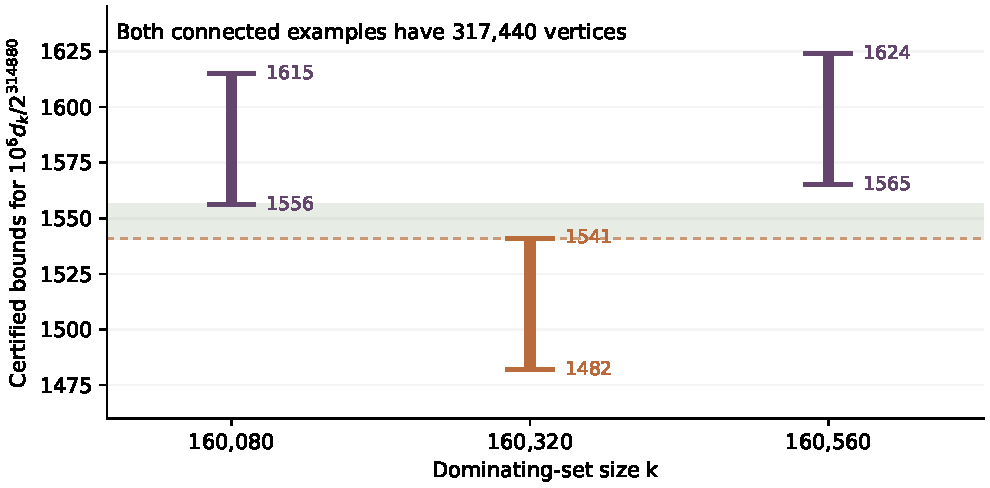
\includegraphics[width=.88\textwidth]{figures/coefficient-bounds.pdf}
\caption{Certified intervals for $10^6d_k/H$ at the three indices, from the integer certificate. The upper end of the middle interval lies below the lower ends of both outer intervals. The intervals hold for both graphs.}
\end{figure}
Since $1541<1556$ and $1541<1565$, the three coefficients form a strict valley. This proves Theorem~\ref{thm:finite}. The valley lies at $160320/317440\approx0.505$ of the order, in the upper half as it must.

\subsection{The average size and the modes of the finite example}
We now locate $\avd(G)$ for $G=G_{128,20}$ and show that no index near it is a global mode. Factoring $(1+z)^P$ out of~\eqref{eq:exactpoly} gives
\[
D_G(z)=(1+z)^P\sum_{S}z^{|S|}\Bigl(\frac{z}{1+z}\Bigr)^{F(S)},
\qquad
\avd(G)=\frac{D_G'(1)}{D_G(1)}=\frac P2+\frac{\tr(T^{m-1}T')\,m}{\tr(T^m)},
\]
where $T(z)$ is the transfer matrix of the sum on the right (it equals~\eqref{eq:T} at $z=1$ after the normalisation by $8^s$ per entry) and $T'$ is its entrywise derivative at $z=1$. Explicitly, with $c=a+b$,
\[
T(z)_{ab}=\binom sb z^{s-b}f_c(z)^s,\qquad f_c(z)=z^3+3z^2+3z\Bigl(\frac z{1+z}\Bigr)^{c}+\Bigl(\frac z{1+z}\Bigr)^{3c},
\]
and $f_c'(1)=9+3\cdot2^{-c}+\tfrac32c\,2^{-c}+\tfrac32c\,2^{-3c}$. All entries of $T$ and $T'$ are nonnegative, so computing $(T+\nu T')^{m}$ over dual numbers ($\nu^2=0$) with all entries rounded down, and again with all entries rounded up, brackets both traces. With $2^{-80}$ rounding this gives
\[
160323.034984\le\avd(G)\le 160323.034985 .
\]
The script also checks the dual-number formula against direct enumeration for four small $(m,s)$.

The bracket~\eqref{eq:bracket} holds for every $k$. Its lower bound at $k=160560$ exceeds its upper bound at every $k$ with $160217\le k\le 160412$, a range checked index by index in exact integers. No such $k$ is a global mode, which proves Theorem~\ref{thm:mean-summary}(b). The two humps of the size distribution sit near $\mu_\cA=160000$ and $\mu_\cC=160640$, and the average lies between them.

\subsection{Reproduction}
The script \texttt{verify\_witness.py} evaluates~\eqref{eq:tracebound} and~\eqref{eq:bracket} with the Python standard library and performs the final comparisons in integers. The power $H=2^{314880}$ is stored as an integer, and the second term of~\eqref{eq:pk} is computed with an exact neighbouring-binomial recurrence. The proof needs neither the full polynomial nor the adjacency matrix of the graph. The script \texttt{check\_extensions.py} computes the average and the excluded range above. The script \texttt{smallcheck.py} enumerates all $2^{20}$ vertex subsets of $G_{2,1}$ and $B_{2,1}$ and compares every coefficient with an inclusion--exclusion formula; \texttt{check\_extensions.py} sums~\eqref{eq:exactpoly} over all variable selections and confirms~\eqref{eq:trace} and the formula for $\avd$ below for $(m,s)=(2,1),(3,1),(4,1),(2,2)$, where the totals of $G_{m,1}$ are $614369$, $480239953$ and $376038400961$. The delivered edge list of $B_{128,20}$ is checked by \texttt{check\_graph.py}.

\section{A computer-free proof for a larger graph}\label{sec:elementary}
This section proves nonunimodality of $G_{2048,128}$ and $B_{2048,128}$ by hand, using a contour-counting bound on the dominating sets outside the two phases and Chebyshev's inequality. The same bound drives Section~\ref{sec:many}.

Divide all counts by $2^P4^h$. For the $i$th block let $u_i$ be the number of bad singletons in $L_i$ and $w_i$ the number of bad triples in $R_i$. After this normalisation a good triple has weight $1$, while the four bad selections of a triple next to $c$ bad singletons have total weight $(3\cdot2^{-c}+2^{-3c})/4\le2^{-c}$; selected and omitted singletons both have weight $1$. So the configurations with given counts have total weight at most
\begin{equation}\label{eq:soft}
\prod_{i=1}^{m}\binom{s}{u_i}\binom{s}{w_i}
\,2^{-\sum_i(u_i w_i+w_i u_{i+1})}.
\end{equation}
This bound drops all interactions except those between neighbouring blocks. Each pure family has normalised mass $U=2^h$.

Fix an integer $q\ge4$. Give the cell $(L_i,R_i)$ the label $L$ when $u_i\ge q$ and $w_i=0$, the label $R$ when $u_i=0$ and $w_i\ge q$, and the label $E$ (exceptional) otherwise. Some configurations of the pure families contain $E$ cells; the bound below covers a superset of the configurations outside the pure families, which is enough. Each specified $L$ or $R$ cell has mass at most $2^s$, and an $E$ cell has mass at most $\omega2^s$, where
\begin{equation}\label{eq:e}
\omega=\omega(s,q)=
2^{1-s}\sum_{j=0}^{q-1}\binom{s}{j}
+2\sum_{j=1}^{3}\binom{s}{j}
\left(\frac{1+2^{-j}}{2}\right)^s
+\left(\frac{25}{32}\right)^s .
\end{equation}
The first term covers cells with fewer than $q$ bad objects on one side and none on the other. For mixed cells, sum first over states in which one count equals $1$, $2$ or $3$, applying the binomial theorem to the other count. When both counts are at least four, $(u-2)(w-2)\ge4$ gives $uw\ge2(u+w)$, which bounds the sum by $(5/4)^{2s}$ before division by $2^s$. Overlaps between these cases only enlarge the bound.

Every passage from an $R$ cell to the next cell labelled $L$ carries a factor at most $\theta=2^{-q^2}$ from the bad pairs on the intervening edge. Set $\kappa=m(m+1)$.

\begin{lemma}\label{lem:arc}
If $\kappa\omega<1$ and $\kappa\theta<1$, the number of dominating sets of $G_{m,s}$ outside $\cA\cup\cC$ is at most $H\rho$, where
\begin{equation}\label{eq:rho}
\rho=\frac{1}{(1-\kappa\omega)(1-\kappa\theta)}-1 .
\end{equation}
\end{lemma}
\begin{proof}
A cyclic labelling with $j$ exceptional cells and $r$ transitions from $R$ to $L$ has weight at most $U\omega^j\theta^r$ in the normalisation~\eqref{eq:soft}. If $j+r>0$, choose the locations of these cells and transitions in at most $m^{j+r}$ ways. Removing the exceptional cells and cutting the chosen transition edges leaves at most $j+r$ intervals, each labelled $L\cdots LR\cdots R$ (either run may be empty), so each has at most $m+1$ labellings. There are therefore at most $\kappa^{j+r}$ labellings. If $j=r=0$, all labels agree, and the configuration lies in $\cC$ (all $L$) or $\cA$ (all $R$). Summing the two geometric series over $j+r>0$ proves the bound.
\end{proof}

\begin{proposition}\label{prop:elementary}
Both $G_{2048,128}$ and $B_{2048,128}$, of order $202\,375\,168$, have nonunimodal domination sequences.
\end{proposition}
\begin{proof}
Take $q=8$. Exact rational evaluation of~\eqref{eq:e} gives $\omega<4.51\cdot10^{-14}$, and~\eqref{eq:rho} gives $\rho<1.9\cdot10^{-7}$. The two phase means and their midpoint are integers, and so is $\Delta/4$. Use three consecutive half-open integer windows of radius $\Delta/4$ centred at these three numbers.

By Chebyshev's inequality and~\eqref{eq:variance}, a phase falls outside its own window, or inside the middle window, with probability at most
\[
\chi=16V/\Delta^2=193/1024 .
\]
The outer windows therefore contain at least $H(1-\chi)$ dominating sets, and the middle window at most $H(2\chi+\rho)$. Since $1-\chi>2\chi+\rho$, the middle sum is the smallest. In the bipartite graph the outer bound becomes $H(1-\chi-2\eta)$ and is still larger.

For three ordered, disjoint integer windows of equal width, a middle sum smaller than both outer sums gives three ordered coefficients with a strict valley: choose a coefficient at least the average in each outer window and one at most the average in the middle window. Hence each sequence is nonunimodal.
\end{proof}

\section{Many peaks}\label{sec:many}
This section proves Theorem~\ref{thm:many-summary}. Gluing gadgets of geometrically increasing size gives $K$ equal-sized families whose mean sizes form an arithmetic progression.

Let $K=2^a$ with $a\ge2$, and put
\[
m=4096K,\qquad s=16\lceil4\log_2K\rceil,\qquad m_i=2^im
\quad(0\le i<a).
\]
Take the $a$ graphs $G_{m_i,s}$ and join all their variable vertices into a single clique. The resulting connected split graph has domination polynomial
\begin{equation}\label{eq:product}
\prod_{i=0}^{a-1}D_{G_{m_i,s}}(z).
\end{equation}
Indeed, each gadget's clauses must be dominated locally. In a gadget with some selected variable, its own clique already dominates all its variables; in a gadget with none, every clause is forced and dominates every variable. Adding edges between the variable cliques therefore changes nothing.

Write $H_i=2^{P_i+3h_i}$ for the phase size of the $i$th gadget and $W=\prod_i H_i$. Choosing one pure family in every gadget gives $K$ product families, each with $W$ members. Their mean sizes are a common constant plus
\[
\Delta_0\sum_{i=0}^{a-1}\varepsilon_i2^i,
\qquad \Delta_0=ms/4,\quad \varepsilon_i\in\{0,1\},
\]
so the $K$ means form an arithmetic progression with step $\Delta_0$, one family per mean. Every product family has variance at most
\[
v=(\tfrac32s^2+s)m(K-1),\qquad
\frac{v}{\Delta_0^2}<\frac1{160}.
\]
Place an integer window of radius $\Delta_0/4$ at every mean, and a window of the same width halfway between each adjacent pair. By Chebyshev, every outer window contains at least $W(1-16v/\Delta_0^2)$ sets. An intermediate window is at distance at least $(r+1/4)\Delta_0$ from the $r$th nearest family mean on either side, so summing Chebyshev's bounds over all families gives at most
\begin{equation}\label{eq:manymiddle}
\frac{2Wv}{\Delta_0^2}\sum_{r\ge0}(r+1/4)^{-2}
\le40Wv/\Delta_0^2 .
\end{equation}
Here the $r=0$ summand is $16$ and the remaining sum is at most $\int_0^\infty(x+1/4)^{-2}\,dx=4$.

Apply Lemma~\ref{lem:arc} to each gadget with $q=\lceil\sqrt s\rceil$. Equation~\eqref{eq:e} gives $\omega=O(s^3)(25/32)^s$, the last term dominating for large $s$, and $\theta\le2^{-s}$. Since $\kappa=O(K^4)$ for every gadget, $s\ge64\log_2K$ and $64\log_2(32/25)>22.7$, every $\rho_i$ is $O(K^{-18})$. Each gadget has at most $H_i(2+\rho_i)$ dominating sets, so the configurations outside all product families number at most
\[
W a\rho_{\max}(2+\rho_{\max})^{a-1}=o(W).
\]
Overlaps between product families only increase the upper sum used in~\eqref{eq:manymiddle}. Each intermediate window is therefore strictly below its two neighbours for large $K$. The exact check in \texttt{check\_extensions.py} shows that the hypotheses of Lemma~\ref{lem:arc} and the window inequalities already hold for $K=4,8,16$; for $K=4$ the outer windows contain at least $0.929W$ sets and the middle windows at most $0.177W$.

For connected bipartite graphs, take the $B_{m_i,s}$, reverse the bipartition of alternate gadgets, and join variable vertices in consecutive gadgets by one edge. These edges respect the bipartition. Every product family remains available up to the union-bound loss $4ms(K-1)2^{-4s}=o(1)$ of the variable-domination failures, and since clause domination still characterises the split product, the split product bounds the new family above. The same window inequalities follow, and every degree is at most $6s+2=O(\log n)$.

The common order is
\[
n=(6s^2+4s)m(K-1)=O(K^2(\log K)^2),
\]
so $K\ge c\sqrt n/\log n$. Choosing a coefficient at least the window average in each outer window and one at most the average in each intermediate window gives $K$ peak regions with strict dips between them. The sequence starts with zeros and ends at $d_n=1$, so the outer high coefficients can be extended to local maxima. For $K=4$, $s=128$ and $n=4\,857\,004\,032$. This proves Theorem~\ref{thm:many-summary}.

\section{Every global mode far from the average}\label{sec:mode}
This section proves Theorem~\ref{thm:mean-summary}(a). A different local gadget gives two families with exactly equal counts and linearly separated sizes. We then note a consequence for sampling.

\subsection{A symmetric sparse interaction graph}
Fix
\[
\varepsilon=10^{-9},\qquad C_0=128\varepsilon^{-2}.
\]
For every sufficiently large integer $m$, there is a bipartite graph $F_m$ with parts $\{L_1,\ldots,L_m\}$ and $\{R_1,\ldots,R_m\}$ such that
\begin{enumerate}[label=(\alph*)]
\item exchanging $L_i$ with $R_i$ for every $i$ is an automorphism,
\item $M_F=|E(F_m)|\le2C_0m$,
\item every pair of subsets $A,B$ in opposite parts with $|A|,|B|\ge\varepsilon m$ spans at least $C_0\varepsilon^2m/8$ edges.
\end{enumerate}
To prove existence, choose each unordered pair $\{i,j\}$ of distinct indices independently with probability $C_0/m$ and put in both edges $L_iR_j$ and $L_jR_i$. For fixed $A,B$, at least $(|A||B|-m)/2\ge\varepsilon^2m^2/4$ distinct unordered pairs could contribute, so the number chosen has mean at least $C_0\varepsilon^2m/4$. The binomial Chernoff bound gives probability at most $\exp(-C_0\varepsilon^2m/32)$ of failing (c). A union bound over at most $4^m$ pairs $A,B$ tends to zero since $C_0\varepsilon^2/32=4>\log4$. Another Chernoff bound gives (b) with probability tending to one, and (a) holds by construction. One may fix $F_m$ as the first graph satisfying these finite conditions in a fixed ordering.

\subsection{Two local gadgets with equal counts}
Each vertex of $F_m$ is a \emph{root}. Give each left root $x$ two private helpers $y_1,y_2$ and, for each $i$, one private vertex $c_i$ adjacent precisely to $x$ and $y_i$. Give each right root $x$ one helper $y$ and three private vertices each adjacent precisely to $x$ and $y$. For every edge $xy$ of $F_m$, add $r_0=256$ distinct \emph{interaction vertices}, each adjacent precisely to $x$ and $y$. Put all roots and helpers into a clique and keep all other vertices independent. This is a connected split graph with
\[
n=10m+r_0M_F\le(10+2C_0r_0)m .
\]
Every independent vertex has degree two, and domination is equivalent to covering every independent vertex, including when the selected clique is empty.

The private configurations of a root are counted by size as follows. If the root is selected, the generating polynomial is $g_+(z)=z(1+z)^4$ for both types. If it is omitted, it is
\[
g_L(z)=(2z+z^2)^2,\qquad g_R(z)=z(1+z)^3+z^3,
\]
so $g_L(z)-g_R(z)=z^2-z$. For either type there are $16$ private choices when the root is selected and $9$ when it is omitted. The conditional mean local sizes, including the root, are
\[
\begin{array}{c|cc}
 &\text{root selected}&\text{root omitted}\\ \hline
\text{left type}&3&8/3\\
\text{right type}&3&23/9 .
\end{array}
\]
For an omitted left root, each helper and its private vertex form a nonempty selected pair, with three possibilities and mean size $4/3$. For an omitted right root, selecting the helper gives eight choices with mean size $5/2$, while omitting it forces all three private vertices.

If $A,B$ are the sets of omitted left and right roots and $\iota=e_{F_m}(A,B)$ is the number of edges between them, then the number of dominating sets with these omitted roots, divided by $16^{2m}2^{r_0M_F}$, is exactly
\begin{equation}\label{eq:rootlaw}
w(A,B)=\lambda^{|A|+|B|}\beta^{\iota},
\qquad \lambda=9/16,\quad\beta=2^{-r_0}.
\end{equation}
Let $Z$ be the sum of these weights. The symmetry of $F_m$ makes this law invariant under exchanging the two parts.

\subsection{Concentration of the omitted roots}
Put $p=\lambda/(1+\lambda)=9/25$ and $\alpha=10^{-3}$. Call a root selection \emph{left-concentrated} when
\[
|B|<\varepsilon m,\qquad ||A|-pm|<\alpha m ,
\]
and define right-concentration by exchanging the parts.

Restricting to $B=\varnothing$ gives $Z\ge(1+\lambda)^m$. Property (c) therefore bounds the probability that both $|A|,|B|\ge\varepsilon m$ by
\[
(1+\lambda)^m\beta^{C_0\varepsilon^2m/8},
\]
which decays exponentially. For $|B|<\varepsilon m$ and $||A|-pm|\ge\alpha m$, discard $\beta^\iota\le1$ and use the binomial tail bound: there are at most $\exp(m\Ent(\varepsilon))$ choices for the small set $B$, whose factor $\lambda^{|B|}$ is at most one, so the probability is at most
\[
2\exp\bigl(-(2\alpha^2-\Ent(\varepsilon))m\bigr).
\]
Since $\Ent(\varepsilon)\le\varepsilon\log(\mathrm e/\varepsilon)<\alpha^2$, this also decays exponentially. Exchanging the parts covers the other side. The two concentrated families are disjoint and each has probability $1/2+O(\mathrm e^{-c_1m})$, for some constant $c_1>0$.

\subsection{Controlling forced interaction vertices}
For any parameter $0<\beta\le1$, condition on all roots except the two ends of a specified edge. The four possible conditional weights have the form
\[
1,\quad\lambda\beta^u,\quad\lambda\beta^v,\quad
\lambda^2\beta^{u+v+1}
\]
for nonnegative $u,v$. Hence the probability that both endpoints are omitted is at most $\lambda^2\beta$, and $\E_\beta\iota\le\lambda^2\beta M_F$. Differentiating the finite partition sum gives
$d\log Z/d\beta=\E_\beta\iota/\beta\le\lambda^2M_F$.
Integrating from $\beta$ to $\sqrt\beta$ yields
\[
\E_\beta\exp\bigl((r_0\log2/2)\,\iota\bigr)
=\frac{Z(\sqrt\beta)}{Z(\beta)}
\le\exp(\lambda^2M_F(\sqrt\beta-\beta)).
\]
With $\zeta=10^{-3}$, Markov's inequality implies
\[
\Prb(r_0\iota\ge\zeta m)
\le\exp\left(-\frac{\zeta\log2}{2}m
+2C_0\lambda^2 2^{-r_0/2}m\right)
\le \mathrm e^{-\zeta(\log2)m/4},
\]
where the last inequality holds for the displayed constants.

\subsection{Size concentration and the mode}
Let $P_0=r_0M_F$. Conditional on $A,B$, the private configurations are independent, and every unforced interaction vertex is an independent fair bit. The conditional mean size is
\[
\mu(A,B)=P_0/2+6m-|A|/3-4|B|/9+r_0\iota/2.
\]
In the left- and right-concentrated families, when $r_0\iota<\zeta m$, this mean is within $m/1000$ of, respectively,
\[
u_L=P_0/2+147m/25,\qquad
u_R=P_0/2+146m/25 ,
\]
which differ by $m/25$. Each local random size has range at most four. Hoeffding's inequality, applied to $2m$ such terms and at most $r_0M_F$ independent bits, gives
\[
\Prb\bigl(||S|-\mu(A,B)|\ge m/1000\mid A,B\bigr)
\le2\exp\left(-\frac{2\cdot10^{-6}m}{32+2C_0r_0}\right).
\]
Hence the intervals $I_L,I_R$ of radius $m/500$ around $u_L,u_R$ each have probability $1/2+O(\mathrm e^{-c_2m})$, and their complement has probability $O(\mathrm e^{-c_2m})$.

Some coefficient has probability at least $1/(n+1)$, so every global mode lies in $I_L\cup I_R$ for all large $m$. The average is within $m/500+o(m)$ of $(u_L+u_R)/2$. Consequently every global mode differs from the average by at least
\[
m/50-2m/500-o(m)\ge3m/200,
\]
a positive constant times $n$.

For a connected bipartite version, delete every clique edge and add one \emph{anchor} vertex adjacent to every root and helper. Place the anchor with the independent vertices in one part, and the roots and helpers in the other. Every choice satisfying the original covering constraints on the independent vertices becomes a dominating set when the anchor is added, because the anchor dominates every root and helper. Omitting the anchor also works exactly when the choice already dominates every root and helper and selects some root or helper (to dominate the anchor). So each original choice has one or two extensions. The two size intervals, enlarged by one, still carry all but exponentially small probability, and their probabilities now lie between $1/3-o(1)$ and $2/3+o(1)$. The average lies within $(u_L-u_R)/6+m/500+o(m)$ of the midpoint $(u_L+u_R)/2$, so every global mode is at distance at least
\[
m/75-2m/500-o(m)\ge m/125
\]
from the average. The new graph has $n+1\le(11+2C_0r_0)m$ vertices and minimum degree two. This proves Theorem~\ref{thm:mean-summary}(a), with
\[
c_{\rm split}=\frac{3}{200(10+2C_0r_0)},\qquad
c_{\rm bip}=\frac{1}{125(11+2C_0r_0)}.
\]

\begin{remark}\label{rem:constants}
These constants are of order $10^{-25}$, and $m$ must be astronomically large for the estimates to apply; the interaction graph is chosen by an existence argument. The proof is written for brevity rather than for good constants. Theorem~\ref{thm:mean-summary}(b) gives an explicit graph instead.
\end{remark}

\subsection{A consequence for sampling}
The same separation slows down the natural local sampler. Single-site Glauber dynamics on the dominating sets of a graph picks a uniform vertex $v$ at each step and replaces $S$ by $S\triangle\{v\}$ when the result still dominates; its stationary law is uniform on dominating sets.

\begin{proposition}\label{prop:slow}
For the split and bipartite graphs of this section, the mixing time of single-site Glauber dynamics on dominating sets is $\mathrm e^{\Omega(n)}$.
\end{proposition}
\begin{proof}
Let $\pi$ be the uniform law, choose an integer $\vartheta$ strictly between the two size intervals, and let $\mathcal S$ be the set of dominating sets of size at most $\vartheta$. One step changes the size by at most one, so every transition from $\mathcal S$ to its complement starts at a set of size exactly $\vartheta$, a set of $\pi$-probability $\phi=O(\mathrm e^{-c_2m})$. Both $\pi(\mathcal S)$ and $\pi(\mathcal S^c)$ are at least $1/3-o(1)$. Start the chain from $\pi$ conditioned on $\mathcal S$. Its law $\mu_t$ satisfies $\mu_t\le\pi/\pi(\mathcal S)$ at every time, because this holds at time zero and the transition matrix is symmetric. Hence $\mu_{t+1}(\mathcal S^c)\le\mu_t(\mathcal S^c)+\phi/\pi(\mathcal S)$, and $\mu_t(\mathcal S^c)\le t\phi/\pi(\mathcal S)$. The total variation distance from $\pi$ at time $t$ is at least $\pi(\mathcal S^c)-t\phi/\pi(\mathcal S)$, which exceeds $1/4$ until $t$ is of order $1/\phi=\mathrm e^{\Omega(m)}$. Some starting state does at least as badly as this starting distribution, and $n=O(m)$.
\end{proof}

\section{Counterexamples with logarithmic minimum degree}\label{sec:highdegree}
This section proves Theorem~\ref{thm:degree-summary}(i). We pad each clause of the basic construction with private filler vertices, which raises the minimum degree to about $\tfrac12\log_2 n$ while keeping the two phases.

Let $t\to\infty$ through integers, set
\[
m=t^2,\qquad s=2^t t^{14},\qquad
h=ms,\quad P=6ms^2,
\]
and give every original clause $t$ new private \emph{filler} vertices, each joined to its clause. In the split version put all fillers and original variables into one clique; the original clauses remain an independent set, each of degree $t+3$.

Fix a selection of the original variables. For a clause already covered by that selection, the clause and its $t$ fillers have $2^{t+1}$ possible selections. For an uncovered clause they have $2^{t+1}-1$, since the selection must be nonempty. These constraints characterise domination of the split graph, including the case of an empty clique selection. If $F$ is the original forced-clause count, the contribution is
\[
2^{(t+1)P}(1-\gamma)^F,
\qquad \gamma=2^{-t-1}.
\]
The two original pure families now have equal size
$H_t=2^{(t+1)P+3h}$.
Their size laws are~\eqref{eq:phaseA}--\eqref{eq:phaseB} with $P$ replaced by $(t+1)P$. Their mean difference remains $\Delta=h/4$, and their variances are at most
\begin{equation}\label{eq:hivariance}
V_t=\tfrac32(t+1)ms^2+ms.
\end{equation}

\begin{lemma}\label{lem:hiphase}
The number of dominating sets outside the two pure families is $o(H_t)$.
\end{lemma}
\begin{proof}
Normalise by $2^{(t+1)P}4^h$, put $q=\lceil s/t^4\rceil$, and treat the $2m$ singleton and triple blocks as the vertices of a cycle in their natural order. A block is \emph{heavy} if it has at least $q$ bad objects. If $k_x$ is the number of bad objects in block $x$, then $F\ge\sum_{xy}k_xk_y$ over adjacent blocks, so the weight is at most the binomial multiplicities times
$\exp(-\gamma\sum_{xy}k_xk_y)$.

If two adjacent blocks are heavy, the total normalised weight is at most $2^{2h}\mathrm e^{-\gamma q^2}$. Its ratio to the pure mass $2^h$ tends to zero, because $\gamma q^2\sim2^{t-1}t^{20}$ while $h=2^t t^{16}$.

If the heavy blocks are pairwise nonadjacent and number at most $m-1$, bound each heavy block by $2^s$ and every light block by
$\sum_{j<q}\binom{s}{j}\le2^{s\Ent_2(q/s)}$.
Summing over at most $2^{2m}$ patterns bounds the ratio to $2^h$ by
\[
2^{-s+2ms\Ent_2(q/s)+2m}=o(1),
\]
since $2m\Ent_2(q/s)=O((\log t)/t^2)=o(1)$.

The only independent sets of $m$ vertices in a cycle of length $2m$ are its two parity classes. Suppose one parity class is entirely heavy. Each bad object on the other parity class has at least $2q$ bad neighbours, costing $\mathrm e^{-2\gamma q}$. Summing all states on the heavy side by $2^h$, the relative contribution with at least one bad object on the other side is at most
\[
(1+\mathrm e^{-2\gamma q})^h-1=o(1),
\]
because $2\gamma q\sim t^{10}$ and $\log h=O(t)$. The configurations with no bad object on the light side are exactly the pure families. The three cases cover every configuration.
\end{proof}

Use three equal-width integer windows centred at the nearest integers to the two pure means and their midpoint, with radius $\lfloor\Delta/8\rfloor$. Equation~\eqref{eq:hivariance} gives
\[
V_t/\Delta^2=\frac{24(t+1)}m+\frac{16}{ms}\longrightarrow0 .
\]
Chebyshev's inequality and Lemma~\ref{lem:hiphase} give outer counts $(1-o(1))H_t$ and middle count $o(H_t)$, so the sequence is nonunimodal.

For a bipartite version, keep the original variables and fillers on the left and the original clauses on the right, and add $t+2$ anchor vertices on the right, each adjacent to every left vertex. Clause domination still imposes the same constraints. In either pure family some original variable is selected, so every anchor is dominated; requiring at least one selected anchor then dominates every left vertex and discards only a fraction $2^{-t-2}$. Counting all anchor selections gives an upper bound, and in the pure families adds an independent $\Bin(t+2,1/2)$ size variable before the all-zero anchor choice is discarded. The same three windows, with their common centre shifted by $(t+2)/2$, give the same strict valley.

The split graph has order $N_t=4ms+(t+1)P$ and the bipartite graph has $N_t+t+2$ vertices. Both are connected. Their minimum degree is exactly $t+3$, attained by the original clauses and, in the bipartite graph, also by the fillers. Finally
\[
\log_2N_t=2t+31\log_2t+O(1),\qquad
\frac{\delta}{\log_2N_t}\longrightarrow\frac12.
\]
The factor $\tfrac12$ arises because the number of clauses grows like $s^2\approx2^{2t}$ while the clause degree is only about $t$. This proves Theorem~\ref{thm:degree-summary}(i).

\section{A sufficient degree criterion}\label{sec:upper}
This section proves Theorem~\ref{thm:degree-summary}(ii) by counting the ways one added vertex can turn a non-dominating set into a dominating one.

For each vertex $v$ put $b_v=|N[v]|=\deg(v)+1$. Let $A_k$ count the pairs $(S,x)$ in which $|S|=k$, $S$ does not dominate, and $S\cup\{x\}$ dominates. Counting all pairs $(S',x)$ with $S'$ a dominating $(k+1)$-set and $x\in S'$ gives the identity
\begin{equation}\label{eq:pivot}
(k+1)d_{k+1}=(n-k)d_k+A_k .
\end{equation}
Since $A_k\ge0$, it gives $d_k\le d_{k+1}$ whenever $n-k\ge k+1$; this is the known rising half \cite[Proposition~2.4]{BB}.

The new ingredient is an upper bound on $A_k$. If $S$ misses $N[v]$ and $S\cup\{x\}$ dominates, then $x\in N[v]$. Charging each pair $(S,x)$ to a missed neighbourhood, and allowing several charges, gives
\begin{equation}\label{eq:Ak}
A_k\le\sum_v b_v\binom{n-b_v}{k}.
\end{equation}
Together with the union bound $d_k\ge\binom nk-\sum_v\binom{n-b_v}{k}$ \cite[Proposition~9]{Omar}, this controls the upper half. For $k\ge\lceil n/2\rceil$,
\[
\frac{\binom{n-b}{k}}{\binom nk}
=\prod_{j=0}^{b-1}\frac{n-k-j}{n-j}\le2^{-b}.
\]
If $\sum_v(b_v+1)2^{-b_v}\le1$, then
\[
A_k\le\binom nk\sum_v b_v2^{-b_v}\le\binom nk\Bigl(1-\sum_v2^{-b_v}\Bigr)\le d_k .
\]
Since $2k\ge n$, identity~\eqref{eq:pivot} gives $(k+1)d_{k+1}\le(n-k+1)d_k\le(k+1)d_k$, so $d_{k+1}\le d_k$. Combined with the rising half, this proves the first statement of Theorem~\ref{thm:degree-summary}(ii); note that $(b_v+1)2^{-b_v}=(\deg v+2)2^{-\deg v-1}$.

\begin{corollary}\label{cor:mindeg}
Every graph on $n\ge4$ vertices with $\delta(G)\ge\log_2n+\log_2\log_2n+1$, and more generally every graph with $n(\delta+2)2^{-\delta-1}\le1$, has a unimodal domination sequence with a global mode at $\lceil n/2\rceil$.
\end{corollary}
\begin{proof}
The function $x\mapsto(x+2)2^{-x-1}$ decreases for $x\ge0$, so $n(\delta+2)2^{-\delta-1}\le1$ implies the criterion. With $L=\log_2n$ and $x=L+\log_2L+1$, we get $n(x+2)2^{-x-1}=(L+\log_2L+3)/(4L)\le1$ whenever $\log_2L+3\le3L$, which holds for $L\ge2$.
\end{proof}
This improves the leading coefficient $2$ in the minimum-degree conditions of Beaton and Brown \cite[Theorem~3.2]{BB} and Omar \cite[Proposition~13]{Omar} to $1$. Theorem~\ref{thm:degree-summary}(i) shows that no condition below $(\tfrac12+o(1))\log_2n$ can force unimodality.

\section{The central mode: sharpness for every large order}\label{sec:central}
This section proves the lower bounds in Theorem~\ref{thm:degree-summary}(iii); the upper bounds follow from Corollary~\ref{cor:mindeg}, which gives $c(n)\le\lceil L+\log_2L+1\rceil$. We construct graphs whose closed neighbourhoods barely overlap. In such graphs many sets miss exactly one closed neighbourhood, each of which can be repaired in many ways, and~\eqref{eq:pivot} then pushes $d_{\lceil n/2\rceil+1}$ above $d_{\lceil n/2\rceil}$.

\begin{lemma}\label{lem:repairs}
Let $G$ have $n$ vertices and maximum degree at most $b$, let every closed neighbourhood have size $b$ or $b+1$, and suppose any two distinct closed neighbourhoods share at most two vertices. Let $k=\lceil n/2\rceil$ and $\xi=(n+4b^2)2^{-b}$. Then
\[
A_k\ge(1-\xi)\sum_{u}b_u\binom{n-b_u}{k}.
\]
\end{lemma}
\begin{proof}
Fix $u$ and let $S$ be a uniform $k$-subset of $V\setminus N[u]$, a set of $n-b_u$ vertices. For $w\ne u$, the event that $S$ also misses $N[w]$ requires $S$ to avoid the $t_w=|N[w]\setminus N[u]|$ vertices of that set, which has probability $\binom{n-b_u-t_w}{k}/\binom{n-b_u}{k}\le\bigl((n-b_u-k)/(n-b_u)\bigr)^{t_w}\le2^{-t_w}$ because $2k\ge n$. If $N[w]\cap N[u]=\varnothing$ then $t_w\ge b$; otherwise $w$ is within distance two of $u$, which happens for at most $b^2$ vertices $w$, and $t_w\ge b-2$. A union bound shows that $S$ misses some other closed neighbourhood with probability at most $n2^{-b}+4b^22^{-b}=\xi$. So at least $(1-\xi)\binom{n-b_u}{k}$ sets of size $k$ have $u$ as their only undominated vertex. Each of them becomes dominating after adding any of the $b_u$ vertices of $N[u]$, and the pairs obtained for different $u$ are distinct.
\end{proof}

\paragraph{Even order.}
Let $n$ be even, $L=\log_2 n\ge20$, and $b=\lfloor L+\log_2L-2\rfloor$. Take two copies of $\mathbb Z/(n/2)\mathbb Z$, called left and right, and join left vertex $x$ to right vertices
\[
x+\sigma_j,\qquad \sigma_j=2b^2j+j^2,\quad 0\le j\le b-2.
\]
This graph is $(b-1)$-regular, so every closed neighbourhood has size $b$. The positive differences $\sigma_i-\sigma_j=(i-j)(2b^2+i+j)$ with $i>j$ are distinct: the quotient on division by $2b^2$ determines $i-j$, and the remainder then determines $i+j$. Since $4\max_j\sigma_j<n$ (we check this below), the differences also remain distinct modulo $n/2$. Thus two vertices in the same part have at most one common neighbour, and two closed neighbourhoods of vertices in opposite parts meet in two vertices when the centres are adjacent and are disjoint otherwise. The graph is connected because $\sigma_0=0$ and $\gcd(\sigma_1,\sigma_2)=1$.

Let $k=n/2$. Lemma~\ref{lem:repairs} gives $A_k\ge nb\binom{n-b}{k}(1-\xi)$. Since $(n/2-j)/(n-j)\ge\tfrac12(1-2j/n)$,
\[
\frac{\binom{n-b}{n/2}}{\binom n{n/2}}=\prod_{j=0}^{b-1}\frac{n/2-j}{n-j}\ge2^{-b}\Bigl(1-\frac{b^2}n\Bigr).
\]
The choice of $b$ gives $4/(nL)\le2^{-b}<8/(nL)$ and $L\le b\le2L$. Hence
\[
\frac{A_k}{\binom nk}\ge\frac{4b}{L}\Bigl(1-\frac{b^2}n\Bigr)\Bigl(1-\frac8L-\frac{32b^2}{nL}\Bigr)
\ge4\Bigl(1-\frac{4L^2}{2^L}\Bigr)\Bigl(1-\frac8L-\frac{128L}{2^L}\Bigr)>2.3 ,
\]
using $L\ge20$ in the last step. Likewise $4\max_j\sigma_j<8b^3\le64L^3<2^L=n$. So $A_k>\binom nk\ge d_k$, and at $n=2k$ identity~\eqref{eq:pivot} reads
\[
(k+1)(d_{k+1}-d_k)=A_k-d_k>0 .
\]
The minimum degree is $b-1$ and $n/2$ is not a global mode, so $c(n)\ge b\ge L+\log_2L-3$.

\paragraph{Odd order.}
Let $n$ be odd, $L=\log_2n\ge40$ and $b=\lfloor L+\log_2L-3\rfloor$. Take the even construction above on $n-1$ vertices with this $b$, put $M=2\max_j\sigma_j+1$, and add one new vertex $v$ on the right, adjacent to the left vertices $0,M,2M,\dots,(b-2)M$. A right vertex has at most one neighbour among these, because two of them differ by at least $M$ (also modulo $(n-1)/2$, since $M<4b^3$ gives $(b-1)M<4b^4\le64L^4<(n-1)/2$ for $L\ge40$; likewise $4\max_j\sigma_j<64L^3<n-1$). Any two closed neighbourhoods still share at most two vertices: $N[v]$ meets $N[x]$ in $\{v,x\}$ for each neighbour $x$ of $v$, meets the closed neighbourhood of a right vertex in at most one vertex, and misses that of every other left vertex; adding $v$ to $N[x]$ and $N[x']$ for two neighbours $x,x'$ of $v$ raises their intersection, previously at most one common neighbour, to at most two. The new vertex has degree $b-1$, its neighbours have degree $b$, and all other degrees are $b-1$, so Lemma~\ref{lem:repairs} applies.

Let $k=(n+1)/2$. Now $n-k=(n-1)/2$, each factor $(n-1-2j)/(2(n-j))$ is at least $\tfrac12(1-2(j+1)/n)$, and
\[
\frac{A_k}{\binom nk}\ge nb\,2^{-(b+1)}\Bigl(1-\frac{(b+1)(b+2)}n\Bigr)(1-\xi)\ge\frac{4b}{L}\Bigl(1-\frac{(b+1)(b+2)}n\Bigr)\Bigl(1-\frac{16}L-\frac{64b^2}{nL}\Bigr)>2,
\]
using $8/(nL)\le2^{-b}<16/(nL)$, $L\le b\le2L$ and $L\ge40$. At $n=2k-1$ identity~\eqref{eq:pivot} reads
\[
(k+1)(d_{k+1}-d_k)=A_k-2d_k>0 .
\]
So $\lceil n/2\rceil$ is not a global mode, the minimum degree is $b-1$, and $c(n)\ge b\ge L+\log_2L-4$. This completes the proof of Theorem~\ref{thm:degree-summary}(iii).

The script \texttt{check\_criteria.py} verifies~\eqref{eq:pivot} and~\eqref{eq:Ak} on all $33\,867$ labelled graphs with at most six vertices, and the distinct-difference property for $4\le b\le79$. The script \texttt{check\_extensions.py} builds small even and odd instances of both constructions and confirms the degrees, connectivity and the intersection property, and evaluates the two displayed lower bounds on a grid of values of $L$.

\section{Open problems, scope and verification}\label{sec:scope}
This section states what the paper leaves open and how its claims were checked.

\paragraph{Open problems.}
\begin{enumerate}[label=(\arabic*)]
\item \emph{The unimodality threshold.} Determine the least $\gamma$ such that minimum degree $(\gamma+o(1))\log_2n$ forces a unimodal domination sequence. Theorem~\ref{thm:degree-summary} gives $\tfrac12\le\gamma\le1$. The factor $\tfrac12$ in our construction comes from its quadratic number of clauses; a gadget with fewer clauses per block might raise it.
\item \emph{Small counterexamples.} Our certified example has $317\,440$ vertices and was chosen for a short certificate, not for small order. A later Evidence Press release treats bounded-degree graphs and certifies a smaller example. How small can a counterexample be?
\item \emph{Trees and forests.} All our examples contain cycles and many vertices of large degree, or a clique. Phase coexistence of the kind used here seems unavailable in trees, and the conjecture for trees remains open \cite{BS,DHP}.
\item \emph{Explicit constants.} Make Theorem~\ref{thm:mean-summary}(a) explicit with a reasonable constant, for example by replacing the random interaction graph with an explicit expander that has the required symmetry.
\item \emph{Universal vertices.} Our split graphs have no universal vertex, consistent with Zhang's theorem \cite{Zhang}. How large must the maximum degree of a counterexample be relative to $n$?
\end{enumerate}

\paragraph{Scope.} The finite results are exact. Theorems~\ref{thm:many-summary}, \ref{thm:mean-summary}(a) and~\ref{thm:degree-summary}(i) are asymptotic; the order at which Theorem~\ref{thm:many-summary} starts is checked exactly, while Theorem~\ref{thm:mean-summary}(a) needs very large orders. Theorem~\ref{thm:degree-summary}(iii) concerns the position of the maximum, not unimodality.

\paragraph{Verification.} The certificate scripts use only integer and rational arithmetic and stop with an error if any check fails, also under \texttt{python -O}. They were rerun from a clean copy, and the main certificate and the transfer identity were recomputed independently in exact arithmetic during internal review. The proofs were checked line by line in AI-assisted internal review. There has been no external peer review and no proof-assistant formalisation.

\paragraph{AI use.} This manuscript was developed with substantial assistance from AI systems, which produced and checked the constructions, proofs, code and text under human direction. The author takes responsibility for the content.

\paragraph{Data and code.} The edge list of $B_{128,20}$, its metadata, the generator \texttt{graph\_family.py} and the checking scripts accompany this paper.

\begin{thebibliography}{99}
\bibitem{AP}
S. Alikhani and Y.-H. Peng.
Introduction to domination polynomial of a graph.
\emph{Ars Combinatoria} 114 (2014), 257--266.
Preprint arXiv:0905.2251 (2009).

\bibitem{BB}
I. Beaton and J. I. Brown.
On the unimodality of domination polynomials.
\emph{Graphs and Combinatorics} 38(3) (2022), article 90.
\url{https://doi.org/10.1007/s00373-022-02487-x}. Preprint arXiv:2012.11813.

\bibitem{BS}
I. Beaton and S. Schoonhoven.
On the unimodality of nearly well-dominated trees.
Preprint arXiv:2411.02288 (2024).

\bibitem{BK}
A. Bhattacharyya and J. Kahn.
A bipartite graph with non-unimodal independent set sequence.
\emph{Electronic Journal of Combinatorics} 20(4) (2013), P11.
\url{https://doi.org/10.37236/3034}.

\bibitem{BO}
A. Burcroff and G. O'Brien.
Unimodality and monotonic portions of certain domination polynomials.
\emph{Discrete Mathematics} 346(9) (2023), 113508.
\url{https://doi.org/10.1016/j.disc.2023.113508}. Preprint arXiv:2110.00709.

\bibitem{DHP}
A. Du, S. Heilman and G. Panova.
Trees and graphs with non log-concave dominating set sequence via AI tools.
Preprint arXiv:2605.02193 (2026).

\bibitem{GZ}
D. Galvin and Y. Zhang.
The domination polynomial of powers of paths and cycles.
\emph{Discrete Mathematics} 350(3) (2027), 115520.
\url{https://doi.org/10.1016/j.disc.2026.115520}. Preprint arXiv:2408.12731.

\bibitem{Omar}
M. Omar.
New perspectives on the unimodality of domination polynomials.
Preprint arXiv:2601.14494 (2026).

\bibitem{Zhang}
S. Zhang.
Domination polynomial is unimodal for large graphs with a universal vertex.
Preprint arXiv:2111.00641 (2021).
\end{thebibliography}
\end{document}
